\section{Equilibrium \& Comparative Statics}
\label{sec:section3} 
\subsection{Steady State Equilibrium and Approximation}\label{sec:section3.1} 
Following from the above, I now present a refined definition for the steady state equilibrium of the market. Such a market configuration requires that two conditions are satisfied. Firstly, it must be the case that the male and female strategies are mutual best responses, meaning that they solve the sex-specific MDP outlined above given the opposite side's strategy and the aggregate platform state. Furthermore, a \textit{consistency check} is required, where the state arising  
\begin{definition}
    A Steady State Equilibrium is defined by a triplet $(\mu^*, \omega^*, \Psi^*)$ such that:
    \begin{enumerate}
        \item $ \mu^*(\theta,b) \text{ attains } V_m(\theta,b), \; \forall\, \theta, b \in \Theta \times \mathcal{B}_m$, given $\omega^*,\Psi^*$
        \item $ \omega^*(\theta,b) \text{ attains } V_w(\theta,b), \; \forall\, \theta, b \in \Theta \times \mathcal{B}_w$, given $\mu^*,\Psi^*$
        \item $\Psi^*$ satisfies Equations \ref{eq:ss1}, \ref{eq:ss2}, and \ref{eq:ss3} given the strategy profile $(\mu^*, \omega^*)$
    \end{enumerate} 
\end{definition}
\begin{comment}
\begin{itemize}
    \item Define and explain concept of SSE
    \item Explain computation via least-squares
    \item Explain main properties (eg. ESS \& uniqueness)
\end{itemize} 
\end{comment}
\subsection{Best Response Analysis}\label{sec:section3.2} 
Using the computational procedures outlined above, a number of insights can be uncovered related to how exogenous parameters affect an agent's best-response swiping curve. The first parameter I analyse is the discount factor, which represents the probability of remaining inside the platform for an additional time period given the exogenous departure process. Despite this, the discount factor is often interpreted as the representative agent's patience, which turns out to be especially intuitive in the SBDA context. The effects of changes in the discount factor on an agent's best-response rule are shown in \autoref{fig:discount-cs}, which makes it evident that as agent's become less patient, they `lower their standards' for potential matches in the platform, shifting their swiping curve downwards. 

\begin{figure}[h] 
    \centering
    \caption{Comparative Statics on the Discount Factor}
    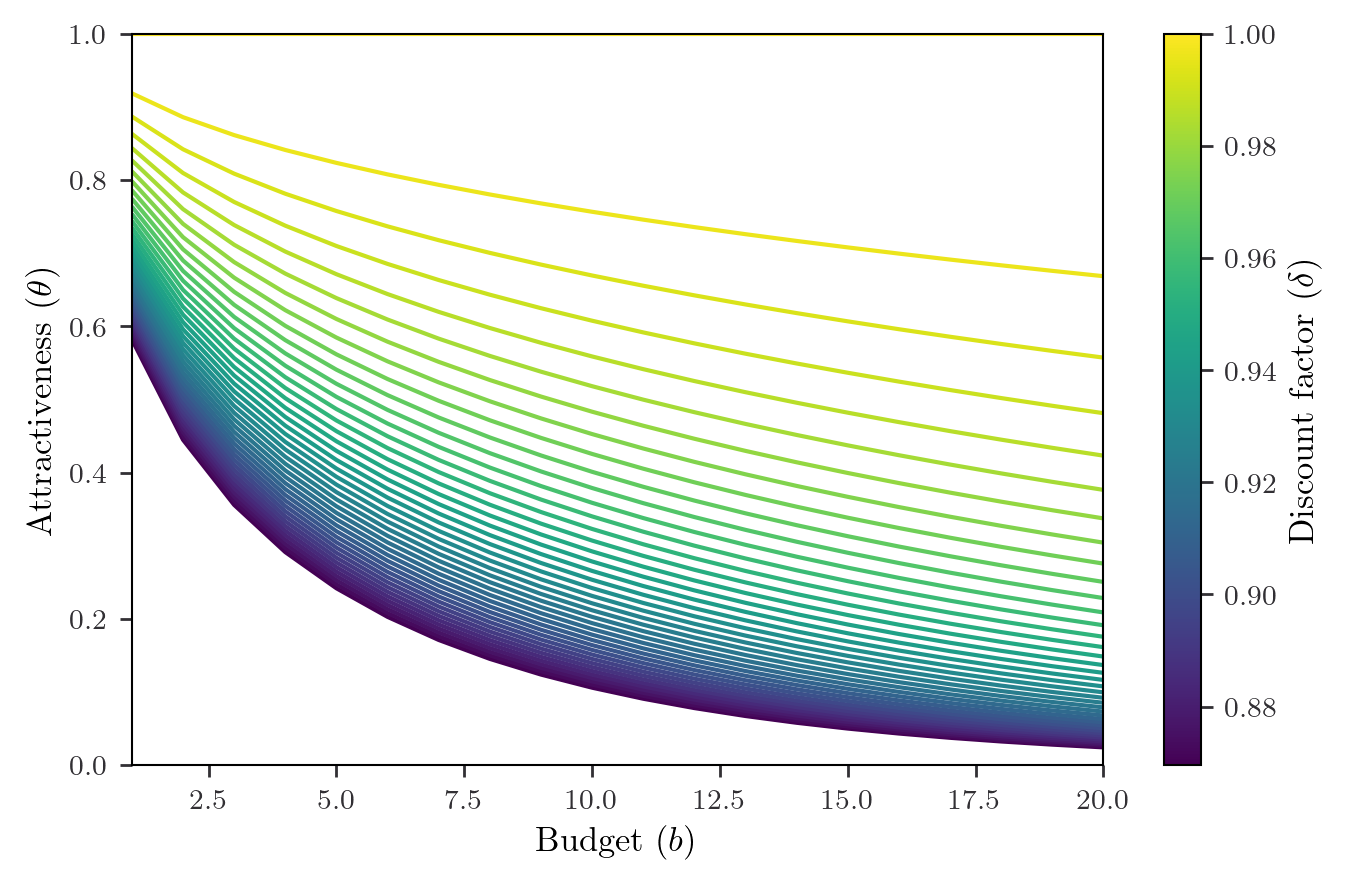
\includegraphics{discount-cs.png}
    \label{fig:discount-cs}
\end{figure}

Despite this, more interesting behaviour arises given the interpretation of a geometrically-distributed platform lifetime process (as explained in \autoref{sec:section2.1}). Under this interpretation, an agent's platform lifetime is of $\frac{1}{1-\delta}$ periods in expectation, meaning that swiping caps significantly higher than this number render the constraint non-binding, thus reverting the game to the trivial case where all agents swipe right in all periods.

Another interesting parameter to examine is the absolute risk aversion of agents, which I choose to interpret as their `desperateness' for matching in the platform. In the platform, risk-averse agents prefer a higher chance of matching (even if these matches yield relatively lower payoffs), whilst risk-loving agents prefer to wait around and save their swipes for high-yield candidates. To perform comparative statics on this parameter, I fix a CARA utility function for agents of the form:
\begin{equation*}
    u(\theta) \,=\, \begin{cases} \left(1-e^{-r\theta}\right)/r & r\neq0 \\ \theta & r=0\end{cases}
\end{equation*}

Where $r$ is the Arrow-Pratt coefficient for absolute risk aversion. With these preferences, I then compute the optimal swiping rule for various different values of $r$ and arbitrary values for other model parameters, with results for this shown on \autoref{fig:risk-cs}. From this, it is evident that as agents become `more desperate' for matches, implied by rising absolute risk aversion, they lower their standards for right-swiping on a candidate, thus shifting their swiping curve downwards (as one would intuitively expect).

\begin{figure}[ht]
    \centering
    \caption{Comparative Statics on Absolute Risk Aversion}
    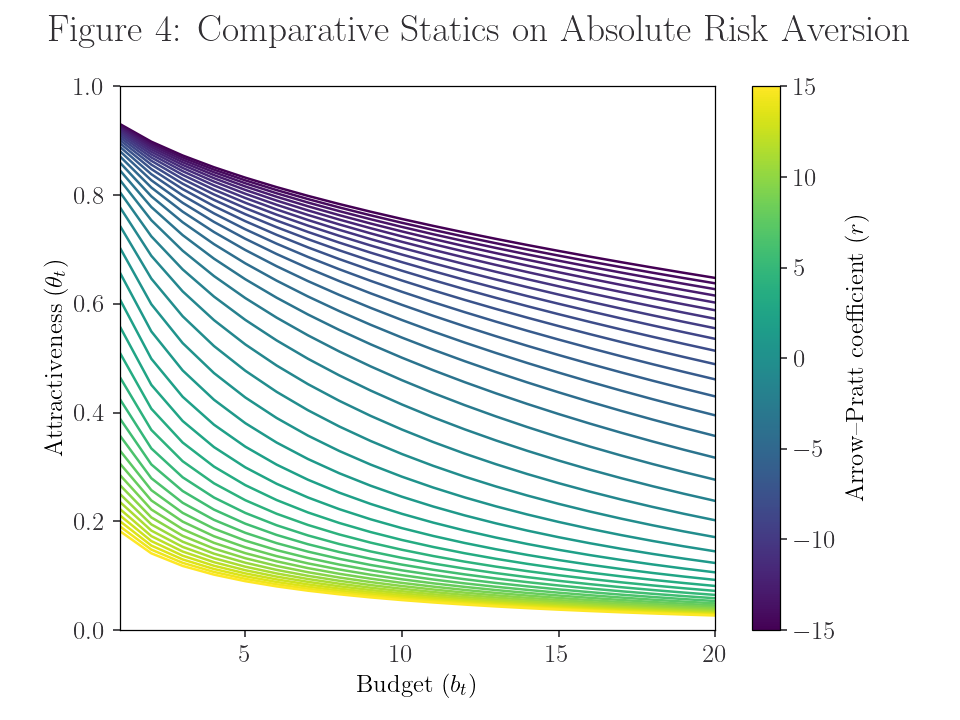
\includegraphics{risk-cs.png}
    \label{fig:risk-cs} 
\end{figure}

\subsection{Market Configuration Analysis}\label{sec:section3.3} 


\begin{comment}
\begin{itemize}
    \item Present CS on individual factors and explain intuitively
    \item These include: patience, risk aversion, distributions  
    \item Present case of gender imbalance... why is it that men always swipe right?
    \item 
\end{itemize} 
\end{comment}